\section{Algorithm Overview}
\label{sec:overview}

\begin{figure*}[t]
  \centering
  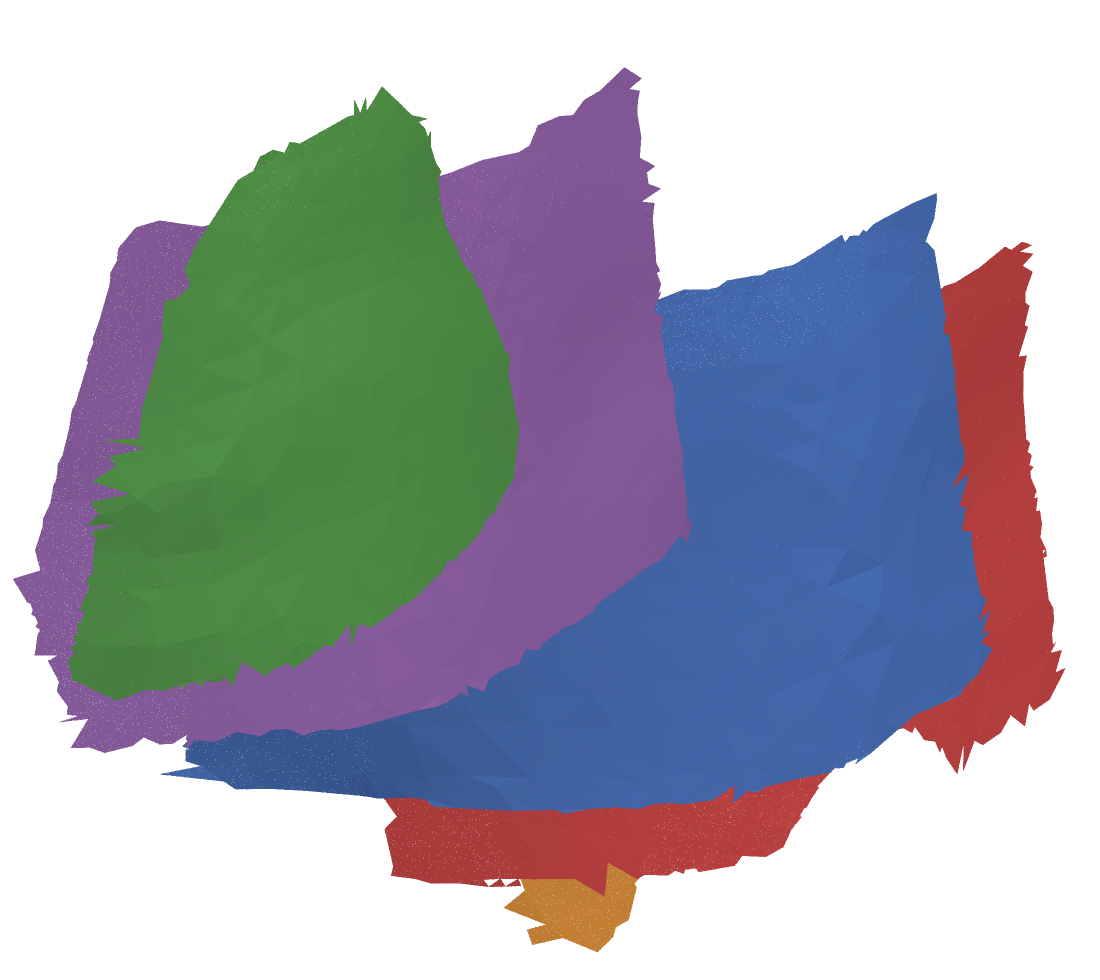
\includegraphics[height=1.13in]{figures/pipe_cube_sheets.png}\hfill
  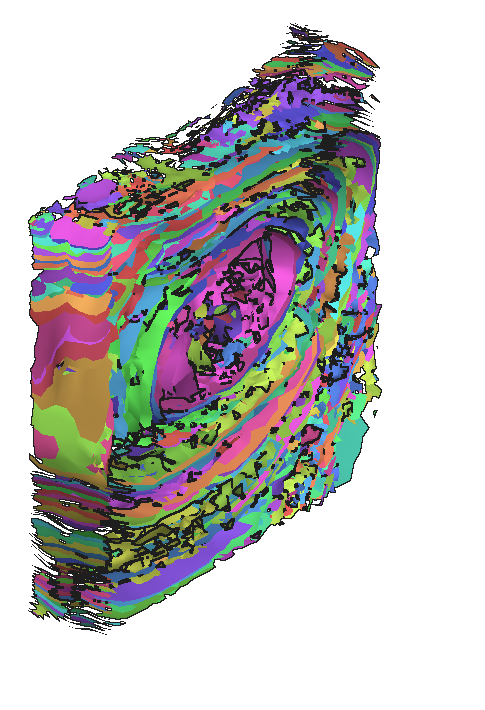
\includegraphics[height=1.13in]{figures/pipe_weld_crop.png}\hfill
  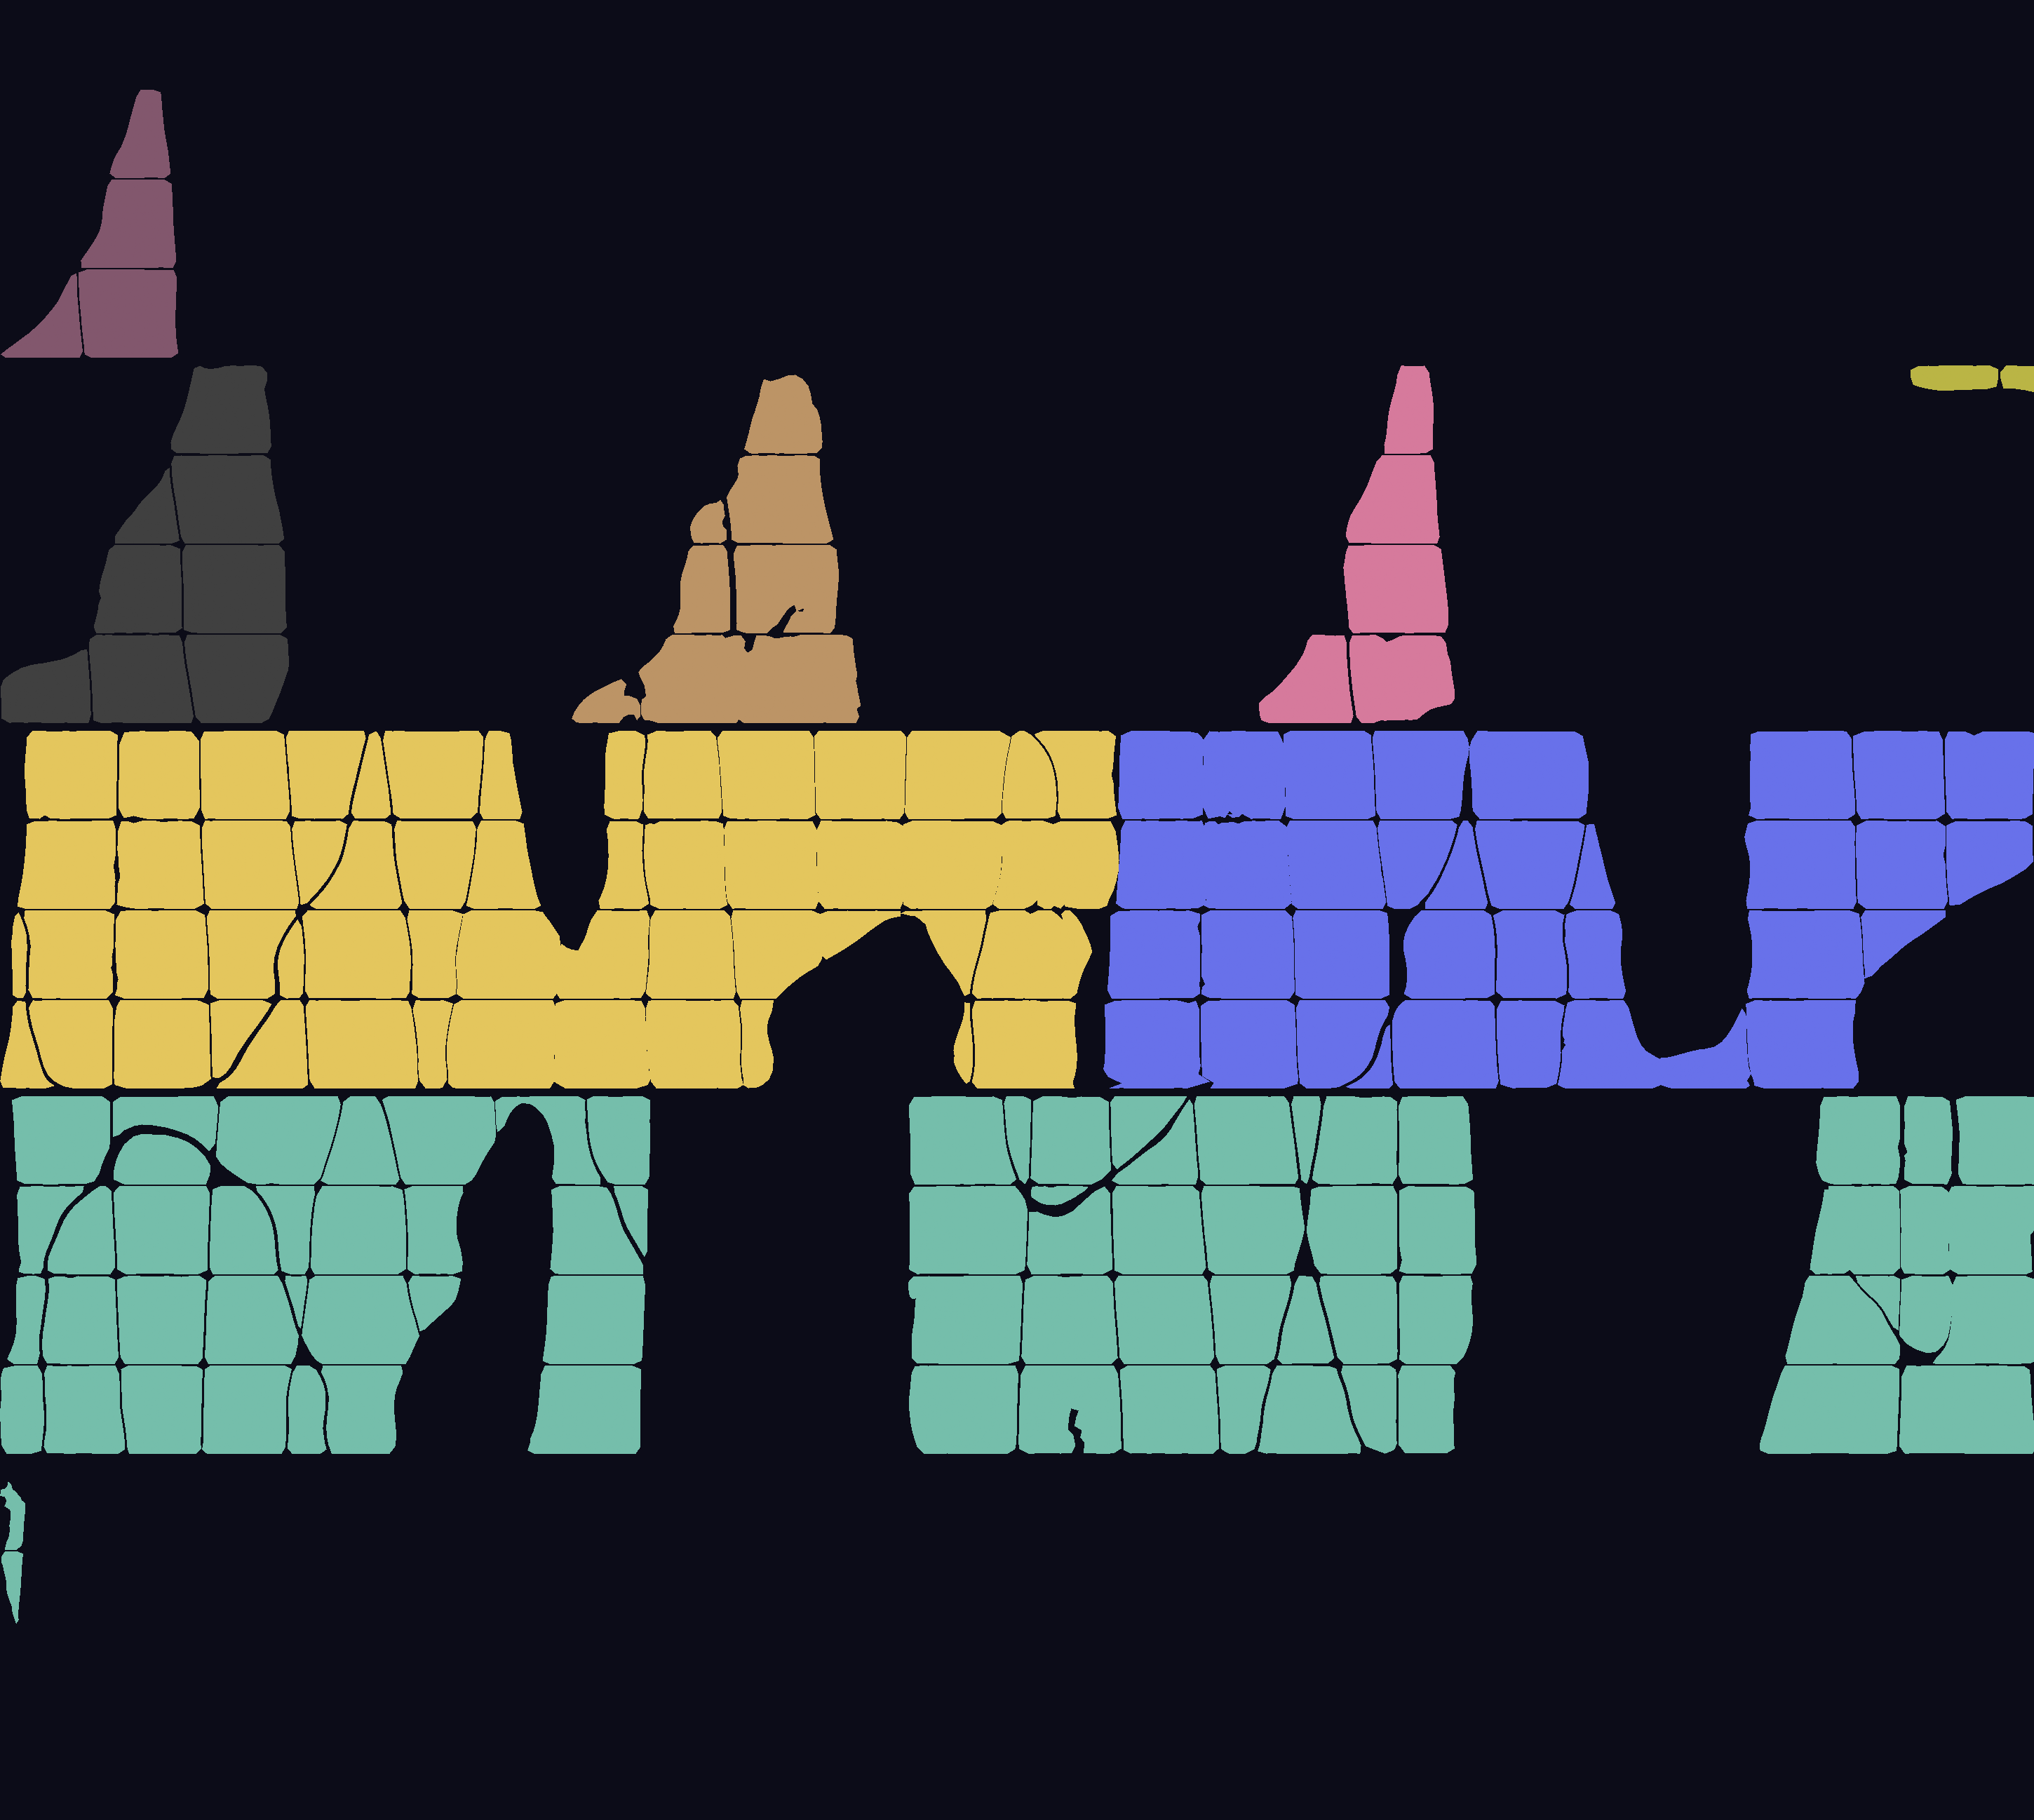
\includegraphics[height=1.13in]{figures/pipe_atlas_crop.png}\hfill
  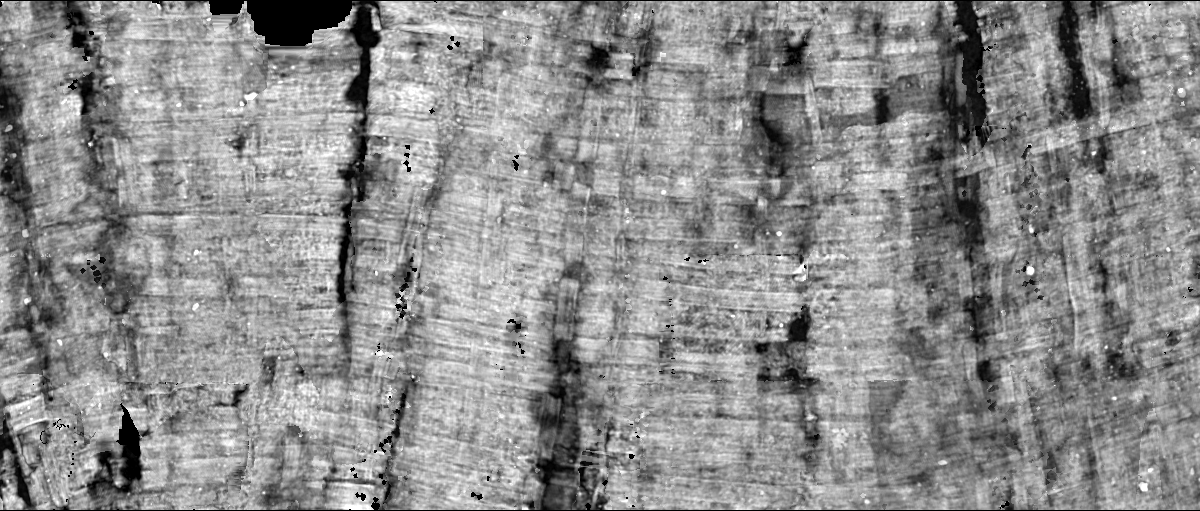
\includegraphics[height=1.13in]{figures/pipe_readback_crop.png}
  \caption{ScrollFiesta overview. Left to right: (a) each cube of thresholded U-Net evidence is collapsed to thin point sheets and meshed into separated, single-sided components (one cube's worth of the reconstructed PHerc0139 fixture shown after level of detail, component-coloured); (b) accepted cubes are CVT-remeshed and welded into a scroll block through refined seam bands; (c) the welded charts are flattened by a slice-domain metric solve, and a discrete winding lift places each welded group on its own wrap in the developed $(u,v)$ domain (detail of the lifted atlas, coloured by welded group); (d) sampling the raw CT volume through the finished map yields the readable sheet, whose continuous fibres validate geometry, winding, and flattening together.}
  \Description{Four panels: a stack of coloured papyrus sheets in one cube, a component-coloured welded scroll block with a spiral cross-section, coloured chart islands laid out in a dark flattened domain, and a grayscale CT texture strip with continuous fibres.}
  \label{fig:pipeline}
\end{figure*}

\subsection{Problem Statement}
\label{sec:problem}

ScrollFiesta takes as input a local array, or remotely stored region, of voxel evidence, normally thresholded to {\em solid} and {\em empty}, together with its world-space origin, voxel scale, cube grid, CT volume, and (for scroll-scale work) the estimated umbilicus and axis. Its output is a triangle mesh with component labels, topology and winding reports; a developed coordinate field or ribbon; sampled CT imagery; and a provenance-bearing \texttt{tifxyz} atlas. It may stop earlier with a mesh-only result, reject a bad cube, or mark downstream geometry unverified when a required gate fails.

Four requirements, established in the introduction, shape the design. First, the useful object is one consistently oriented side of an open sheet, so every stage must construct and preserve single-sided open manifolds rather than the watertight boundaries standard reconstruction produces. Second, a full scroll comprises tens of thousands of cubes, so every stage must operate on a small domain plus a fixed-radius halo and compose deterministically across cube boundaries. Third, a single wrong join --- one short edge connecting surfaces a full turn apart --- can invalidate everything downstream, so a stage that cannot certify its output must quarantine it rather than emit plausible-looking geometry. Fourth, the correct flattened layout is subject to a global, integer-valued winding constraint that no local distortion energy on the surface can express, so parameterization must jointly solve discrete and continuous unknowns rather than minimize distortion alone.

\subsection{Method Pipeline}
\label{sec:pipeline}

Mesh construction proceeds in five stages (Fig.~\ref{fig:pipeline}a,b; per-cube stages in Fig.~\ref{fig:cube_stages}). {\em Extraction} (Sec.~\ref{sec:percube}) guards each cube against degenerate predictions, collapses its voxel evidence to thin point sheets with a moving least-squares estimator, orients the sheets consistently, and meshes them with a guarded ball-pivoting front. {\em Topological repair} (Sec.~\ref{sec:cleanup}) severs thin necks and overlaps, splits pinches, fills clean interior holes, and opens non-separating handles, re-projecting and re-meshing each separated piece from its original voxel points. {\em Level of detail} (Sec.~\ref{sec:cvt}) remeshes each sheet by a restricted CVT, producing near-isotropic triangulations at a uniform budget. {\em Welding} (Sec.~\ref{sec:weld}) joins adjacent cubes through locally refined seam bands under winding gates, then recoarsens the bands by pinned CVT/RVD without disturbing the audited topology. Finally, topology and winding {\em audits} decide whether each welded sheet may be parameterized at all, and on which trust path.

Parameterization then solves for a mixture of discrete and continuous variables. The continuous variables are the developed coordinates $(u,v)$ of every vertex, where $u$ is metric developed length and $v$ is position along the scroll axis; the discrete variables are the integer winding depths of {\em charts} --- connected mesh components, in practice one cube's sheet each --- whose physically welded groupings must land exactly one circumference apart from their inner neighbours. An initial continuous field comes from a slice-domain metric solve anchored by a calibrated spiral prior (Sec.~\ref{sec:unwrap}); winding order alone is an unreliable predictor of scroll topology, so this field is only a starting point. A deterministic tabu search then owns the integers, moving charts and whole welded groups between winding depths, while a continuous re-registration owns the metric, restoring seam agreement with the chosen depths held fixed; the two alternate until no chart moves (Fig.~\ref{fig:pipeline}c). The selected map is rasterized against the CT and cleaned in the parametric domain --- overlap quilting, RAW-guided snap, seam registration, and a collision-audited ribbon fit (Sec.~\ref{sec:repair}) --- before the atlas and its CT read-back are assembled (Fig.~\ref{fig:pipeline}d) and handed off on an explicitly verified or unverified path (Sec.~\ref{sec:integration}).

Sections~\ref{sec:percube}--\ref{sec:repair} describe each stage in detail. Throughout, we state each energy in the form the implementation optimizes; Appendix~\ref{app:terms} collects the precise definition of every term, the default constants, and the complete tabu-search procedure, so that each stage can be reproduced without reading the source.
